%*******************************************************************************
%***************************** Cellular Automata Chapter ***********************
%*******************************************************************************
\chapter{Cellular Automata}
\label{ch:CA}
\dictum[Richard Feynman]{There are many interesting phenomena … which involve a mixture of physical phenomena and physiological processes, and the full appreciation of natural phenomena, as we see them, must go beyond physics in the usual sense. We make no apologies for making these excursions into other fields, because the separation of fields, as we have emphasized, is merely a human convenience, and an unnatural thing. Nature is not interested in our separations, and many of the interesting phenomena bridge the gaps between fields.}%
\vskip 1em

%\section{Introduction}\label{cellularAutomataIntroduction}
\lettrine[lines=4]{P}{hysical} system are usually composed by many components that interact in a complex net of causes and consequences that is often hard or impossible to describe in its entirety analytically.
Even if each single components is simple, extremely complex behaviors emerge naturally due to the cooperative effect of many components. Much has been discovered about the nature of the components in natural systems, but little is known about the way those components interacts as the overall complexity is observed.
Such systems are often described by partial differential equation, which are hard to solve analytically especially when they are non-linear and consequently require alternative, or approximate solutions (see Chapter \ref{ch:FDM}).
\begin{figure}
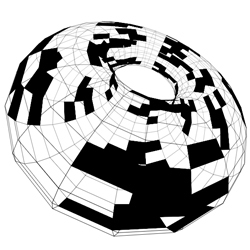
\includegraphics[scale=0.8]{./images/CA_FDM/torus-2}
\caption{3D cellular automata with toroidal cellular space.}
\label{torus}
\end{figure}
This chapter introduces \textit{Cellular Automata} that,  have been proved to be suitable for the modellation and simulation of a wide class of complex physical systems, in particular those ones constructed from \textbf{many identical} components, each (ideally) simple, but together capable of complex behaviour\cite{Toffoli1984,toffoli1987}.
As can be seen from the number of papers in literature  cellular automata have been applied in a wide range of classes of problems from gas\cite{Frisch1986} and fluid turbulence\cite{Succi1991} simulation to macroscopic phenomena\cite{Gregorio1999} like epidemic spread\cite{Sirakoulis2000}, snowflakes and lava flow\cite{dspataro_sciara:2017,Crisci2004,Spataro2010}.
CA were first investigated by \textit{S. Ulam} working on growth of crystals using
lattice network and at the same time by \textit{J. Von Neumann} in order to study
self-reproduction\cite{Neumann1966}; it was not very popular until the 1970 when
the famous \textit{Conway's} game of life\cite{conway1970} appeared, and since then  they have been widely studied from  a theoretical view point until they were proved capable of computational universality\footnote{ Logical gates can be simulated using the simple rules of the \textit{Game of Life} combining special patterns as \textit{gliders} and \textit{guns}}\cite{Thatcher1970}. They have been mainly adopted, after 1980's, as a computational parallel model due to their intrinsically parallel nature\cite{Margolus1986}.


\section{Informal Definition}

A \emph{cellular automata} (CA) is a mathematical model that
consists of a discrete lattice of sites  and a value, the state, that is
updated in a sequence of subsequents discrete timestamps (steps) according to some  rules that depend on a neighbor sites of the cell. Hence CA describe systems whose the overall behavior and evolution may be exclusively described on the basis of local interactions\cite{wolfram1984}, property also called \textit{centrism}.
The most stringent and typical characteristic of the CA model is the restriction
that the local function does not depend on the time $t$ or the cell site $i$: a cellular automaton has homogeneous space and time behavior. It is for this reason that ca are sometimes referred to as \textit{shift-dynamical} or \textit{translation invariant} systems. From another point of view we can say that in each lattice site resides a  deterministic finite (state) automaton (DFA)\cite{Hopcroft:2006:IAT:1177300} that take as input only the states of the cells in its neighborhood (see \ref{amod3Automata} and section\ref{DFA}).

\subsection{Cellular space dimension and geometry}
The cellular space is a \emph{discrete} $d$-dimensional lattice of sites (see
figure \ref{spazioCellulare}).
For $1D$ automaton the only way to discretize the space is in a one-dimensional
grid. For automaton with dimensionality higher than 1 the shape of each cell can
be different than squared. In $2D$ tessellation for example, each cell can be
hexagonal or triangular, and each tessellation presents its own advantages and disadvantages. For instance the squared can be easily visualized on a screen as each cell is easily mapped onto a pixel.}, but may present problems of anisotropy for some kind of fluid simulations as in the case of the \textit{HPP} model for fluid simulation\cite{Frisch1986}. An Hexagonal tessellation can solve the anisotropy problem\cite{wolfram1986} but presents obvious graphical challenges. Often, to avoid complications due to a boundaries, periodic boundary conditions are used, so that a two-dimensional grid is the surface of a torus as shown in Figure \ref{torus}.

\subsection{Neighborhood}
The evolution of a cell's state is function of the states of the neighborhood's
cells. The geometry and the number of cells that are part of the neighborhood
depends on the tessellation type, but it has to have three fundamental
properties:
\begin{enumerate}
  \item \textbf{Locality}: it should involve only a \textit{limited} or \textit{finite} finite number of cells.
  \item \textbf{Invariance}: it should not be changed during the evolution.
  \item \textbf{Homogeneity}: it has to be the same for each cell of the
  automaton.
\end{enumerate}
Typically, the neighborhood of a cell ``surrounds'' the cell itself. For $1D$ cellular automata, neighborhood are identified with a number $r$ called
\textit{radius}\cite{wolfram1983}. A $r=2$ identifies
$n=2r+1$ cells in a 1D lattice: the central cell plus the
right and left cells. Typical 2D cellular space neighborhood are the those of
\textit{Moore} and \textit{J. Von Neumann} neighborhood. The number of cells in the Moore neighborhood of range $r$ is the odd squares $(2r+1)^2,$ the
first few of which are 1, 9, 25, 49, 81, and so on as $r$ is increased.
Von Neumann's one consist of the central cell plus the cell at north, south,
east, and west of the central cell itself. Moore's ($r=1$)
one add  the farther cells at north-east, south-east, south-west and north-west
(see figure \ref{mooreNeigh}).


\begin{figure}
	\centering
	\caption{Examples of cellular spaces. (a) 1-D, (b) 2-D squared cells,
		(c) 2-D hexagonal cells, (d) 3-D cubic cells.}\label{spazioCellulare}
	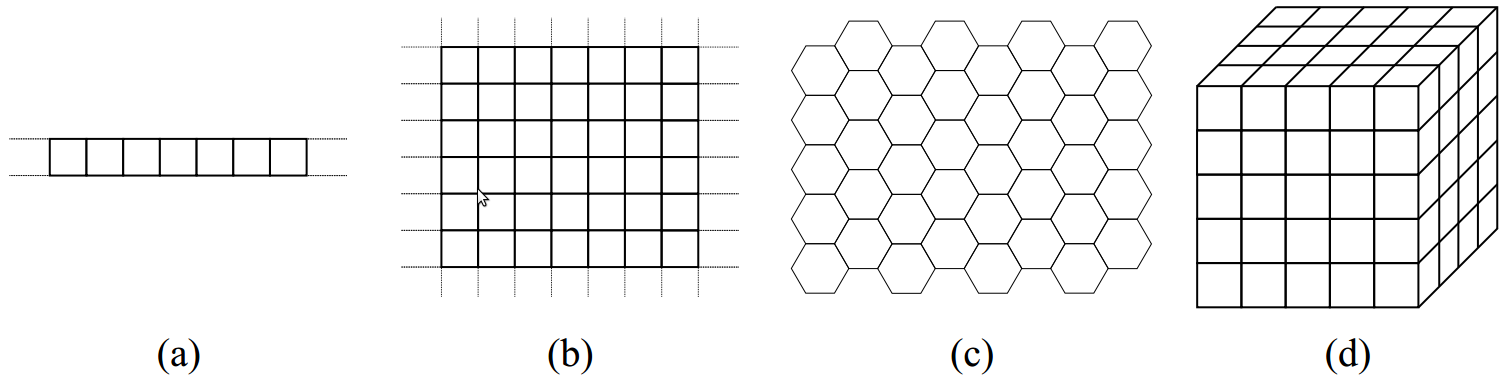
\includegraphics[scale=0.23]{./images/CA_FDM/spazioCellulare}
\end{figure}

\begin{figure}
\centering
\caption{Examples of different kind of neighborhood with
different radius values.}\label{mooreNeigh}
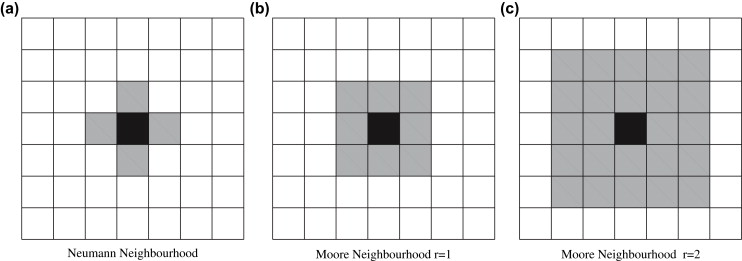
\includegraphics[width=1.0\textwidth]{./images/CA_FDM/mooreNeigh}
\end{figure}

\subsection{Transition Function}
The evolution of the cell's state is specified in the so called \textit{transition function} that is applied at the same time and on each cell. Usually the transition function is \textit{deterministic} and usually defined by a look-up table only when the total number of state for each cell is small, otherwise the resulting table would have enormous size because the number of possible state transition is exponential in the number of states. Alternatively, a transition function is defined by an algorithmic procedure that may be probabilistic, in the case of \textit{stochastic cellular automata}\cite{Arrighi:2013:SCA:2637657.2637659}.

\section{Formal Definition}
Cellular automata are dynamic discrete in time, space and state models, defined by a lattice of cells each containing a finite state automaton.

\subsection{Finite State Automaton}\label{DFA}
Also known as deterministic finite automata (DFAs) or as deterministic finite
state machines, DFAs are among the simplest and better studied computational models.
A DFA is a theoretical model of computation with limited capability. It can only recognize regular languages (the family of languages in the third category of the \textit{Chomsky} classification and that can be obtained by regular expressions) and can only be in one of the finite number of states at a time, namely the \textit{current state}. Its state can change in response of the input taken by a
transition function, describe all possible state changes, and of the current state.
\begin{table}
\scalebox{1.2}{
\begin{tabular}{|c|ccccc|}\hline
\(\delta\) & \(a\) & \(b\) & \(c\) & \(d\) & \(e\) \\ \hline
\(q_0\) &\(q_0\) &\(q_0\) &\(q_2\) &\(q_1\) &\(q_1\)\\  
\(q_1\) &\(q_1\) &\(q_3\) &\(q_1\) &\(q_1\) &\(q_1\)\\  
\(q_2\) &\(q_3\) &\(q_2\) &\(q_2\) &\(q_0\) &\(q_1\)\\  
\(q_3\) &\(q_0\) &\(q_1\) &\(q_1\) &\(q_0\) &\(q_1\) \\ 
\hline 
 \end{tabular}
}
 \caption{Tabular representation of a DFM transition function}
 \label{tab:tabularTransitionFunction}
\end{table} 
It is a much more restrictive model in its computational capabilities than a Turing
machines, for example it is possible to prove that it is not possible for a DFA to determine whether the input consists of a prime number of symbols,
but they are still powerful enough to solve simpler problems, and hence to recognize
simpler languages, as for example the following: $L=\{w \in \{0,1\}^*\}$, the language composed by strings with an even number of $0$ and $1$; they are only capable
to recognize languages in the class $3$ of the \textit{Chomsky} classification\cite{Chomsky:1956}. Infact it can be proven the for each language $L$ accepted by a DFA exists a grammar $L_G$ s.t. $ L=L_G$ i.e. $L_G$ generates $L$,
but they fail for example, in accepting \emph{context-free} languages.

Formally, a DFA is defined as a 5-tuple:
\[M = <Q,\Sigma,\delta,q_0,F>\] 
where:
\begin{itemize}
  \item \textit{Q} is a finite, nonempty, set of states.
\item $\Sigma$ is the alphabet
\item $ \delta : Q \times \Sigma \longmapsto Q  $ is the
transition function, also called next-state function, and can be represented in
tabular form  as  in \ref{tab:tabularTransitionFunction}
\item $q_0 $ is the initial (or starting) state :
$ q_0 \in  Q $
\item  $F $ is the set, possibly empty, of final states:
$ F \subseteq Q $

\end{itemize}
Note that we can also assume that $F$ is composed by a single state i.e. $\left\vert{F}\right\vert=1$ because a DFA can always transformed into another one that accepts exactly the same set of strings and has only one final state. The transformation consists in adding an additional state $q_f$, and for each of the previous final states $q_i \in
F$ a new rule of the type $\delta(q_i,*)=q_f, * \in I $ is added to the transition function.

A run of DFA on a input string $u = a_0,a_1,\ldots,a_n$ is a
sequence of states  $ q_0,q_1,\ldots,q_n$ s.t.
$q_i  \overset{a_i}{\longmapsto} q_{i+1} $,
$ 0 \leq i < n$. For each pair of two states
and a input the transition function deterministically returns the next DFA's
state i.e.  $q_i=\delta(q_{i-1},a_{i}) $.
For a given string $\textit{w}\in \Sigma^* $, the DFA has a
unique run (because of its deterministic nature), and is it said that it \textbf{accepts} $w$ if the last state $q_n \in F$. A DFA recognizes the
language $L(M)$ consisting of \textit{all} strings it accepts.

Figure \ref{amod3Automata} shows an example of a DFA represented graphically as a graph where nodes are the states and the labeled edges are the possible state transitions from a state $u$ to a state $v$.
Note that, because the automaton is deterministic, it is not possible for two
edges with the same label to point to two different nodes.
In this example, $ \Sigma = \{a,b\}$ is the alphabet, $ Q = \{t_0,t_1,t_2\}$ is the set of states, $ q_0 = t_0$ is the initial state and $ F = \{t_0\} $, is the set of final or accepting states and the transition function is s.t. accepts the language  generated by regular expression $E=\{b^*ab^*ab^*a\}$.
When the automaton is executed on the input string $s=\{aaabba\}$ at the beginning of the execution, at time $t=0$ the DFA is in the initial state $t_0$ and the first
symbol of $s$, $a$ is read.
The transition function is applied once per each symbol of $s$
i.e. $\left\vert{s}\right\vert$ times. The only rule that matches 
the current state $t_0$ and the current input $a$ is $\delta=(t_0,a)=t_1 $ hence the new state of the DFA becomes $t_1$. 
The DFA accepts the string only if the current state is in the set of final states $F$ when it has consumed the input in its entirety.
$s$ is not accepted by the DFA described in the Figure\ref{amod3Automata} because
at the end of the computation the reached state is $t_1$ that is not a final state, as shown in the following execution trace:
 \[
 t_0\overset{\delta(t_0,a)}
 {\longmapsto}t_{1}\overset{\delta(t_1,a)}
 {\longmapsto}t_{2}\overset{\delta(t_2,a)}
 {\longmapsto} t_{0}\overset{\delta(t_0,b)}
 {\longmapsto}t_{0}\overset{\delta(t_0,b)}
 {\longmapsto}t_{0}\overset{\delta(t_0,a)}
 {\longmapsto} t_{1}
\]
On the input $S^1=\{abababb\}$, instead, the DFA accepts as shown in the following execution trace:
 \[
 t_0\overset{\delta(t_0,a)}
 {\longmapsto}t_{1}\overset{\delta(t_1,b)}
 {\longmapsto}t_{1}\overset{\delta(t_1,a)}
 {\longmapsto} t_{2}\overset{\delta(t_2,b)}
 {\longmapsto}t_{2}\overset{\delta(t_2,a)}
 {\longmapsto}t_{0}\overset{\delta(t_0,b)}
 {\longmapsto}t_{0}\overset{\delta(t_0,b)}
 {\longmapsto}\mathbf{t_{0}}
\]
\begin{figure}
\begin{center}
  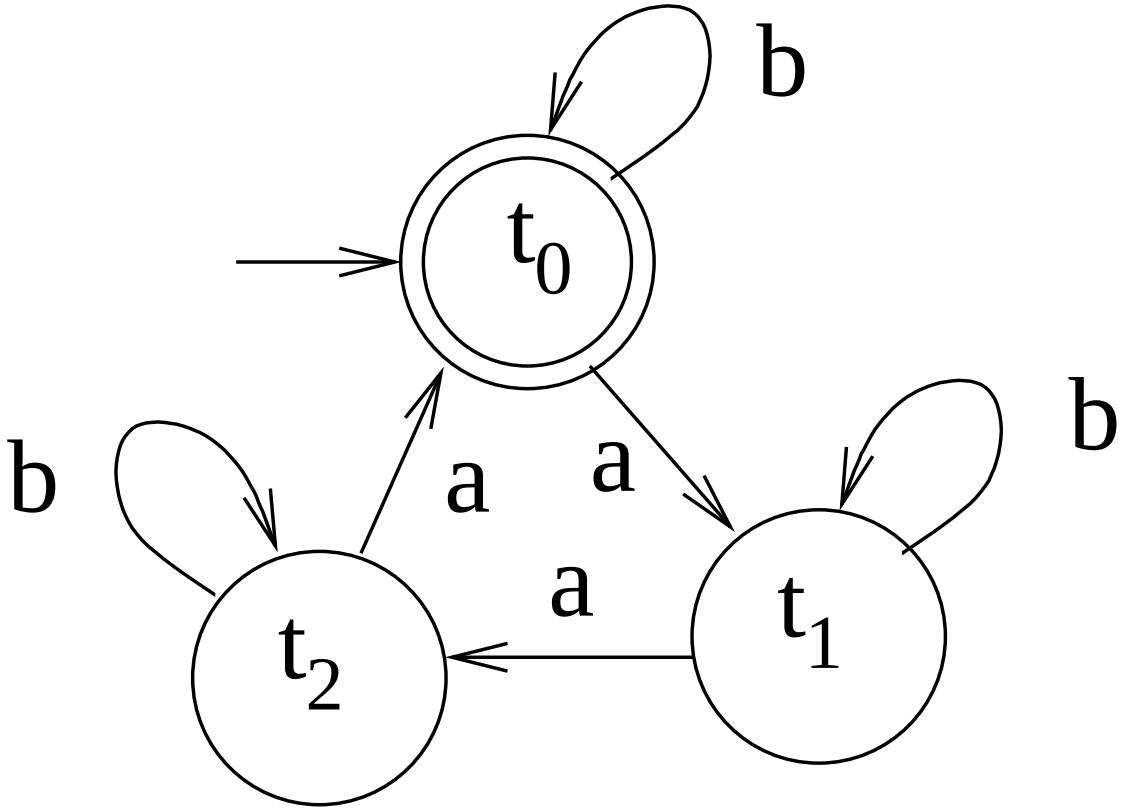
\includegraphics[scale=0.17]{./images/CA_FDM/amod3Automata}
  \caption[Graph representation of a DFA.]{Graph representation of a DFA an that accepts the following language: $\{b^*ab^*ab^*a\}$.}
  \label{amod3Automata}
\end{center}
\end{figure}


\section{Homogeneous Cellular Automata}\label{homogeneousCellularAutomata}
Formally a CA $A$, is defined as  quadruple $ A=<Z^d,X,Q,\sigma>$
where:
\begin{itemize}
  \item $\mathbb{Z}^d=\{i=(i_1,i_1,\ldots,i_d)\mid i_k \in
  \mathbb{Z}, \forall k=1,2,\ldots,d \}$ is the set of cells of the $d$-dimensional  Euclidean space.
  \item $X$ is the neighborhood, or neighborhood template; a
  set of $m$ $d$-dimensional vectors (one for each neighbor)
  \[\xi_j=\{\xi_{j1},\xi_{j2},\ldots,\xi_{jd}\} \;,\: 1\leq j \leq m\] that
  defines the set of the neighbors cells of a generic cell
  $i=(i_1,i_1,\ldots,i_d)$
  \[
  N(X,i)=\{i+\xi_0,i+\xi_2,\ldots,i+\xi_d\}
  \] where $\xi_0$ is the \textit{null vector}. $\xi_0$ ensures that the
  cell $i$ is always in its own neighborhood.  Cell $i$ is refeered as to \emph{central cell}.

\item Q is the finite set of states of the elementary automaton EA.
  
  \item $\sigma=Q^m \rightarrow Q $ is the transition
  function of the EA. $\sigma$ must specify
  $q_k \in Q $ as successor  state of the central cell.
  If there are $m$ cells in the neighborhood of the central
  cell including itself, then there are
  ${\left\vert{Q}\right\vert}^m$ possible neighborhood's
  state configuration. It  means that there are
  ${\left\vert{Q}\right\vert}^{{\left\vert{Q}\right\vert}^m}$
  possible transition functions. Plus we can see that the tabular definition of
  the next-state function is unsuitable for practical purpose. It should have
  $\left\vert{\sigma}\right\vert={\left\vert{Q}\right\vert}^m$
  entries, an exceedingly large number.
  \item $\tau=C \longrightarrow C \longmapsto
  \sigma(c(N(X,i))) $ where 
  where $C=\{c \colon Z^d
  \rightarrow Q\}$
  is called the set of the possible configuration and 
  $
  C(N(X,i)))$ is the set of states of the neighborhood of \textit{i}.
\end{itemize}
As an example, consider a $2$D cellular automaton, a
generic cell $c=(10,10)$ in its cellular space $Z^2$, 5 cell states  ${\left\vert{Q}\right\vert}=5$ with Moore's neighborhood  $X$ defined as follows:
\begin{gather*}
X=\{\xi_{0},\xi_{1},\xi_{2},\xi_{3},\xi_{4},\xi_{5},\xi_{6},\xi_{7},\xi_{8}\}
=\\ \{(0,0),(-1,0),(0,-1),(1,0),(0,1),(-1,-1),(1,-1),(1,1),(-1,1)\}
\end{gather*}
The set of cells belonging to the neighborhood of $c=(10,10)$ is:
\begin{gather*}
V(X,c)=\{(0,0)+c,(-1,0)+c,(0,-1)+c,(1,0)+c,(0,1)+c,(-1,-1)+c,(1,-1)\\
+c,(1,1)+c,(-1,1)+c= \{(10,10),(9,10),(10,9),(11,10),(10,11),(9,9),(11,9),(11,11),(9,11)\}
\end{gather*}
The total number of entries of a tabular definition of a
transition function, taken from the set of all the ${\left\vert{Q}\right\vert}^{{\left\vert{Q}\right\vert}^{\left\vert{X}\right\vert}}=
5^{5^9}=5^{1953125}$ possible transition functions, is  ${\left\vert{Q}\right\vert}^{\left\vert{X}\right\vert}=
5^9=1953125$.



\section{Elementary cellular automata}
The  simplest kind of CA are the so called \textit{elementary} cellular
automata, widely studied by \citeauthor{wolfram1983} in \cite{wolfram1983}. They are defined as a $1$-dimensional periodic array $\{C_i \mid 1\leq i \leq N, C_i \in \{0,1\} \}$ where $N$ is the size of the automata. Each cell can only take one of two possible states, i.e. zero ($0$) or one ($1$).
The transition function depends on the nearest neighbors of, i.e. on cells within a radius $r=1$ from, the central cell, thus involving a total of $2r+1=2\times1+1=3$ cells (central, right and left ones).
Since there are only $2\times2\times2\times=2^{2r+1}=2^3=8$ possible state configurations for
the aforementioned neighborhood, there can only be a total of $2^{2^3}=2^8=256$ possible elementary automata, each of which may be uniquely mapped and to a $8$-bit binary number\cite{wolfram2002}, as shown in Table \ref{wolframcodeGeneral} and Section \ref{sec:wolfram_code}.

\subsection{Wolfram's code}
\label{sec:wolfram_code}
The generic transition function  $F(C_{i-1},C_i,C_{i+1})$ is
defined by a look-up table of the form stated in Table \ref{wolframcodeGeneral} which also shows an example of an instance of a particular function the rule $110$ which is the most important one.
\citeauthor{Cook2004} proved universal computational power of the $110$-th elementary CA, as conjuctured in 1985 by Wolfram himself, which is arguably the simplest Turing complete system \cite{wolfram2002}.

\begin{table}
\caption[Encoding of a transition function for a generic elementary CA to a $8$-bit binary number.]{Encoding of a transition function for a generic elementary CA to a $8$-bit binary number. The transition function rules are firstly ordered according to the neighborhood pattern. Then each value of the right hand side of the $i$-th rule is interpreted as the $i$-bit of a binary number.  The instance $110$ of the Wolfram's elementary CA is shown in the right side of the table.}
\centering
\begin{tabular}{l}
\label{wolframcodeGeneral}

\hfill \\
\hline
  $F(1,1,1)=\{0,1\}$  \\
  $F(1,1,0)=\{0,1\}$  \\
  $F(1,0,1)=\{0,1\}$  \\
  $F(1,0,0)=\{0,1\}$  \\
  $F(0,1,1)=\{0,1\}$  \\
  $F(0,1,0)=\{0,1\}$  \\
  $F(0,0,1)=\{0,1\}$  \\
  $F(0,0,0)=\{0,1\}$  \\
\hline
\end{tabular}
\quad
$\overset{instance}{\longrightarrow}$
\begin{tabular}{l}

\label{wolframcoderule}
\hfill \\
\hline
  $F(1,1,1)=0$  \\
  $F(1,1,0)=1$  \\
  $F(1,0,1)=1$  \\
  $F(1,0,0)=0$  \\
  $F(0,1,1)=1$  \\
  $F(0,1,0)=1$  \\
  $F(0,0,1)=1$  \\
  $F(0,0,0)=0$  \\
\hline
\end{tabular}
\end{table}
Wolfram's code\cite{wolfram1983,wolfram2002} can be is easy to determine given that 
it is possible to sort neighborhoods patters in non-decreasing order (if interpreted as $3$-bits) i.e. $(111=7),(110=6),(101=5)$ etc. using the following procedure:
\begin{enumerate}
  \item Rules are sorted according to the neighborohood
  \item For each configuration, the state which the given cell will take in the subsequent iteration, is specified
  \item The next-iteration state of the $i$-th rule is interpreted as the $i$-th bit of a binary number, which is then converted in base $10$.
\end{enumerate}


\subsection{Wolfram's classification}
	Despite their simple definition the mathematical analysis of elementary CA is not straightforward. A first attempt to classify CA was attempted by \citeauthor{wolfram2002} \cite{wolfram2002}. He proposed a set of four classes for their
classification that is still the most popular method of CA classification even if they
suffer from a degree of subjectivity.
Classification is based only on \textit{visual valuations}, which are obviously subjective. 
A more rigorous definition of these classes is given in \cite{culik1998} where \citeauthor{culik1998} proves that deciding whether an automaton lies in a specific one out of four Wolfram's classes is an undecidable problem.

Wolfram's classes are defined as follows:
\begin{enumerate}[I]
  \item these CA have the simplest behavior; almost all initial conditions
  result in the same uniform initial state (\textbf{homogeneous state}).
  \item different initial conditions yield different final patterns, but
  these different patterns consist of an arrangement of a certain set of
  structures, which stay the same forever or repeat themselves within a few
  steps (\textbf{periodic structures}).
  \item the observed behavior is more complicated and appears random, but
  patterns are still present (often in the form of \textit{triangles})(\textbf{chaotic pattern}).
  \item in some respects these are the most complicated class; these behave
  in a manner somewhere in between class II and III, exhibiting sections
   of both predictable patterns and randomness (\textbf{complex structures}).
\end{enumerate}
Wolfram  observed that the behavior of a meaningful class of Cellular Automata
by performing computer simulations of the evolution of the automata starting
from random configurations. He suggested that the different behaviors of
automata in his classes seems to be related to the presence of different types
of attractors.
In Figure \ref{class34} some elementary automata are divided in their respective classes.
 \begin{figure}
 \caption[Example of elementry CA in Wolfram's four classes.]{Examples of Wolfram's class 1 (a,b),  2 (c,d), 3 (e,f) and 4 (g,h) elementary cellular automata}
 \label{class34}
\centering
    \begin{subfigure}[b]{0.25\textwidth}
		\centering
		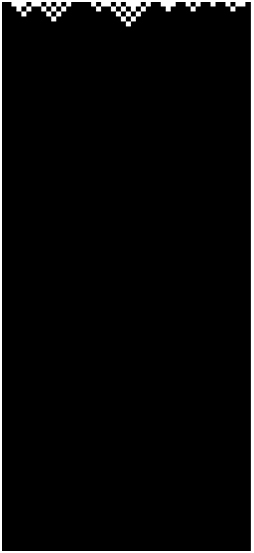
\includegraphics[scale=0.32]{./images/CA_FDM/rule250}
   \caption[]{Rule 250}
   \end{subfigure}%
    \begin{subfigure}[b]{0.25\textwidth}
		\centering
		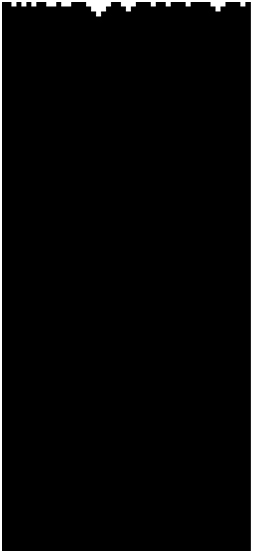
\includegraphics[scale=0.32]{./images/CA_FDM/rule254}
		\caption[]{Rule 254}%
   \end{subfigure}%
       \begin{subfigure}[b]{0.25\textwidth}
   	\centering
   	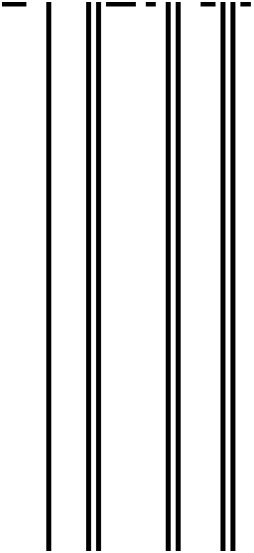
\includegraphics[scale=0.32]{./images/CA_FDM/rule4}
   	\caption[]{Rule 4}%
   \end{subfigure}%
   \begin{subfigure}[b]{0.25\textwidth}
   	\centering
   	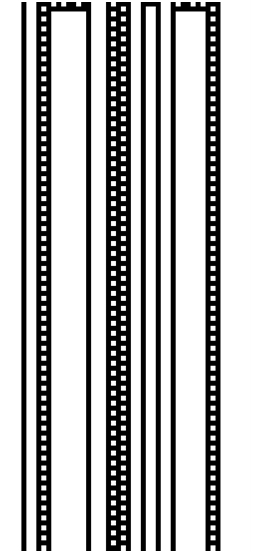
\includegraphics[scale=0.32]{./images/CA_FDM/rule108}
   \caption[]{Rule 108}%
   \end{subfigure}%
   \\
   	\begin{subfigure}[b]{0.25\textwidth}
   		\centering
   		\label{fig:first}
   		
   		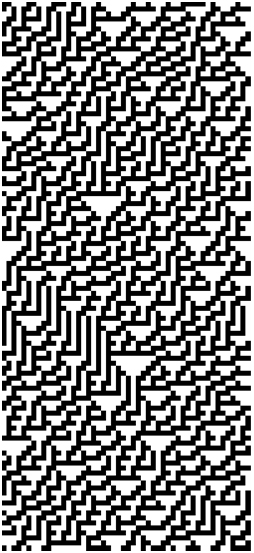
\includegraphics[scale=0.32]{./images/CA_FDM/rule30}
   		\caption[]{Rule 30}%
   	\end{subfigure}%
   	\begin{subfigure}[b]{0.275\textwidth}
   		\centering
   		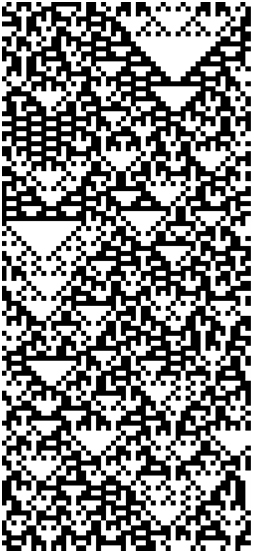
\includegraphics[scale=0.32]{./images/CA_FDM/rule90}
   		\caption[]{Rule 90}%
   	\end{subfigure}%
   		\begin{subfigure}[b]{0.25\textwidth}
   			\centering
   			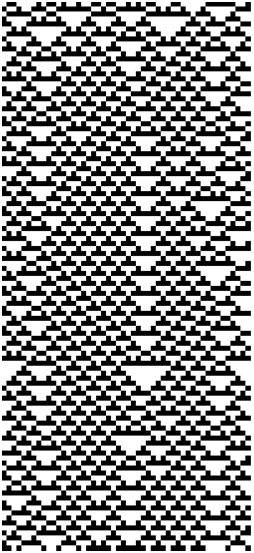
\includegraphics[scale=0.32]{./images/CA_FDM/rule54}
   			\caption[]{Rule 54}%
   		\end{subfigure}%
   		\begin{subfigure}[b]{0.25\textwidth}
   			\centering
   			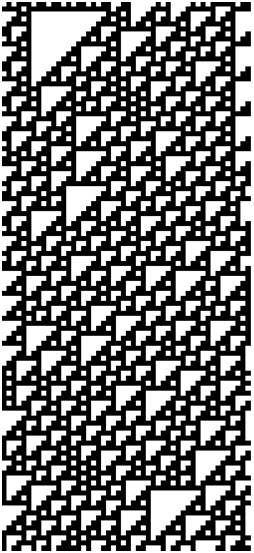
\includegraphics[scale=0.32]{./images/CA_FDM/rule110}
   			\caption[]{Rule 110}%
   		\end{subfigure}%
   	
   	
\end{figure}
It is clear from these examples that automata from class $1$ end up very quickly having the same value i.e. in a \textit{homogeneous state} while automata
from class 2 in a simple final periodic patterns.
Class 3 appear to be completly chaotic and non-periodic while automata from class 4 have
a mixed behaviour where complex-chaotic structures are locally propagated.
\subsection{At the edge of Chaos}
Class 4 automata are at \emph{the edge of chaos} and give a good metaphor for
the idea that the \textit{interesting} complexity like the one exhibit by
biological entities and their interactions or analogous to the phase transition
between solid and fluid state of the matter, is in equilibrium between
stability and chaos\cite{Langton1990}.
\begin{quotation}
\em Perhaps the most exciting implication (of CA representation of biological
phenomena) is the possibility that life had its origin in the vicinity of a
phase transition and that evolution reflects the process by which life has
gained local control over a successively greater number of environmental
parameters affecting its ability to maintain itself at a critical balance point
between order and chaos.\\
(\textit{\textbf{Chris Langton} - Computation at the edge of chaos.
Phase transition and emergent computation - pag.13}).
\end{quotation}


Langton in his famous paper, \textit{Computation at the edge of chaos: phase
transition and emergent computation}\cite{Langton1990},was able to
identify, simply parametrizing the rule space, the various CA classes, the
relation between them and to ``couple'' them with the classical complexity classes.
He introduced the parameter $\lambda$\cite{LangtonThesis1990} that, informally, is simply
the fraction of the entries in the transition rule table that are mapped to the
not-quiescent state.
The definition of the $\lambda$ parameter is as follows:
\[\lambda=\frac{K^N-n_q}{K^N}\]
where:
\begin{itemize}
  \item $K$ is the number of the cell states
  \item $N$ the arity of the neighborhood
  \item $n_q$ the number of rules mapped to the quiescent
  state $q_q$
\end{itemize}

\begin{figure}
\centering
\caption{Relation between lambda parameter and the CA
behaviors-Wolfram's classes.}\label{lambdaWolframClass}
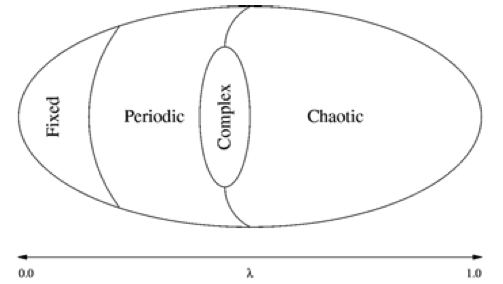
\includegraphics[scale=0.4]{./images/CA_FDM/edgeofchaos}
\end{figure}
Langton's major finding was that a simple measure such as it correlates with the
system behavior: as it goes from $0$ to $ 1-\frac{1}{K}$, the most
homogeneous and the most heterogeneous rules table scenario, respectively, the average
behavior of the system goes from freezing to periodic patterns to chaos and functions with an average value of $\lambda$ are being on \emph{on the edge}\cite{Langton1990}(see Figure \ref{lambdaWolframClass}).
\citeauthor{Langton1990} studied a entire family of totalistic CA with $k=4
$ and $N=5$ and having $\lambda$ varying in $[0,0.75]$. He was able to determine that values
of $\lambda\approx0.45$ raise up to class 4 cellular automata.
Computational system must to provide fundamental properties if it is
to support computation. Only CA \emph{on the edge} show these properties on
manipulating and store information data.
The properties that a computational system must provide are:
\begin{description}
  \item[Storage] \hfill \\
   the ability of the system of preserving information for
arbitrarily long times
  \item[Transmission] \hfill \\
  the propagation of the information in the
form of signals over arbitrarily long distance
  \item[Modification] \hfill \\
	the modification of one or more signals.
\end{description}
Storage is coupled with less entropy of the system, but transmission and
modification are not. Few entropy is associated with CA of class 1 and 2 while
higher entropy with class 3. Class 4 is something in between, the cells cooperate
and are correlated to each other, but not too much otherwise they would be overly
dependent with one mimicking the other. Moreover they are very dependent to the initial
configuration opening to the possibility to encode programs in it.

\section{Game of life}
\label{sect:GOL}
CA are suitable for representing many physical, biological, social and other
natural phenomena.
But they have proved to be a good tool to study under which condition a
physical system expose the basic operations 
to  support computation in all its aspects and requirements. Game of life is a famous 2D
cellular automaton of the '70s well studied for its universal
computation capacity, which has been perhaps proved.

\subsection{Definition} 
The Game of Life (GOL) is totalistic CA.
A totalistic cellular automaton is a one in which the rules depend only on the total, or equivalently, the average, of the values of cells in the neighborhood. 
GOL can be thought as an infinite two-dimensional orthogonal and regular grid of square cells, each taking one of two possible states, \emph{dead} or \emph{alive}.
Every cell interacts with the nine adjacent neighbors belonging to the Moore neighborhood. At each time step, one of the following transitions occur:
	\begin{itemize}
	\item \emph{Birth}: if the cell is in the state \textbf{\textit{dead}} and
	the number of alive neighbors is \textbf{\textit{3}}, then the cell state
	becomes alive (1) .
	\item \emph{Survival}: if the cell is in the state \textbf{\textit{alive}}
	and the number of alive neighbors is \textbf{\textit{2 or 3}}, then the cell
	state is still alive (1) .
	\item \emph{Death}: If the cell is in the state \textbf{\textit{alive}} and
	the number of alive neighbors is \textbf{\textit{less than 2 or higher
			than 3}}, then the cell state becomes dead (0).
\end{itemize}
The initial configuration of the system specifies the state (dead
or alive) of each cell in the cellular space. The evolution of the
system is thus obtained by applying the aforementioned transition function rules \textbf{simultaneously} to every cell in
the cellular space, so that each new configuration depends on the
one at the current step. The rules continue to be applied
repeatedly to create further generations.

Formally the Game of Life automaton is be defined as follows:
$$Life = < R, X, Q, \sigma >$$ where:
\begin{itemize}
	\item $R$ is the set of cells, forming a two-dimensional toroidal cellular space. A generic
	cell in $R$ is individuated by means of a pair of integer
	coordinates $(i, j)$ s.t. $0 \leq i < i_{max}$ and $0 \leq j <
	j_{max}$ where $i_{max},j_{max}$ are the sizes of $R$ in the horizonthal and vertical directions, respectively.
	The first coordinate, $i$, represents the row, while
	the second, $j$, the column. The cell at coordinates $(0,0)$ is
	located at the top-left corner of the computational grid
	(cf. Figure \ref{spazioCellulare}).
	
	\item $X = \{(0,0), (-1, 0), (0, -1), (0, 1), (1, 0), (-1,-1),
	(1,-1), (1,1), (-1,1)\}$ is the Moore neighborhood pattern. The
	coordinates of neighbors of $(i,j)$ are given by:
	$$N(X, (i, j)) = $$
	$$= \{(i, j)+(0,0), (i, j)+(-1, 0), \dots, (i, j)+(-1,1)\} =$$
	$$= \{(i, j), (i-1, j), \dots, (i-1,j+1)\}$$ .
	A subscript	can be used to index cells belonging to the
	neighborhood. Let $|X|$ be the number of elements in X, and $n
	\in \mathbb{N}$, $0 \leq n < |X|$; the notation
	$$N(X, (i, j), n)$$
	represents the coordinates of the $n$-th neighbor of  $(i,j)$.
	Thereby, $N(X, (i, j), 0) = (i, j)$, i.e. the
	central cell, $N(X, (i, j), 1) = (i-1, j)$, i.e. the first
	neighbor, and so on (cf. Figure \ref{mooreNeigh}b).
	
	\item $Q = \{0, 1\}$ is the set of cell states, $0$ representing the
	dead state, $1$ the alive one.
	
	\item $\sigma : Q^9 \rightarrow Q$ is the deterministic cell
	transition function. It is composed by a single elementary process,
	which implements the aforementioned evolution rules.
\end{itemize}
The Game of Life belongs to the class 4 of the Wolfram's taxonomy, because (quoting the words of Wolfram)
\say{rich and complex structures, stable blocks and moving patterns come into existence even starting from a completely random configuration}. 
Among many patterns and blocks appearing in the GOL, one of the most common is the so called \emph{glider} (see Figure \ref{fig:glider}) that is a periodic pattern with a period of $5$ steps that is capable of moving into the cellular space and thus of transmitting information.
\begin{figure}
\centering
\caption[GOL execution example.]{An execution of the Game of Life. Many common patterns are visible as blikers, gliders and beacons.}
\label{gameoflife}
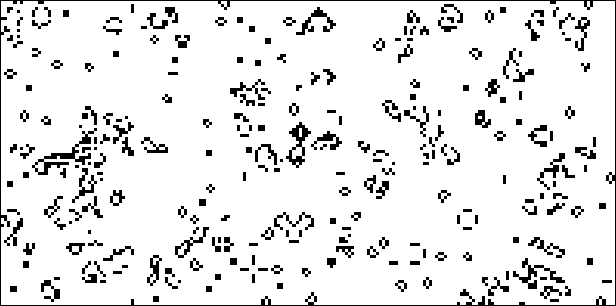
\includegraphics[width=1.0\textwidth]{./images/CA_FDM/game-of-life}
\end{figure}

\subsubsection{Game of life as Turing machine}
Every CA con be considered as a device capable of supporting computation where the
initial configuration  encodes an input string (the source code of a program ). At
some point in time, the current configuration can be interpreted as the result of the
computation and decoded into an output string. As mentioned in Section
\ref{DFA}, not all the computational devices have the same (computational) power.
So which is the one of the game of life? GOL is proved to be capable of universal computation.
Therefore the Game of life is computationally equivalent to a Turing machine\cite{berlekamp1982}.
\begin{figure}
\centering
\caption[The \textit{Glider} block in the Conway's game of life.]{Glider in Conway's game of life.}
\label{fig:glider}
\setlength{\fboxrule}{1pt}%
\fbox{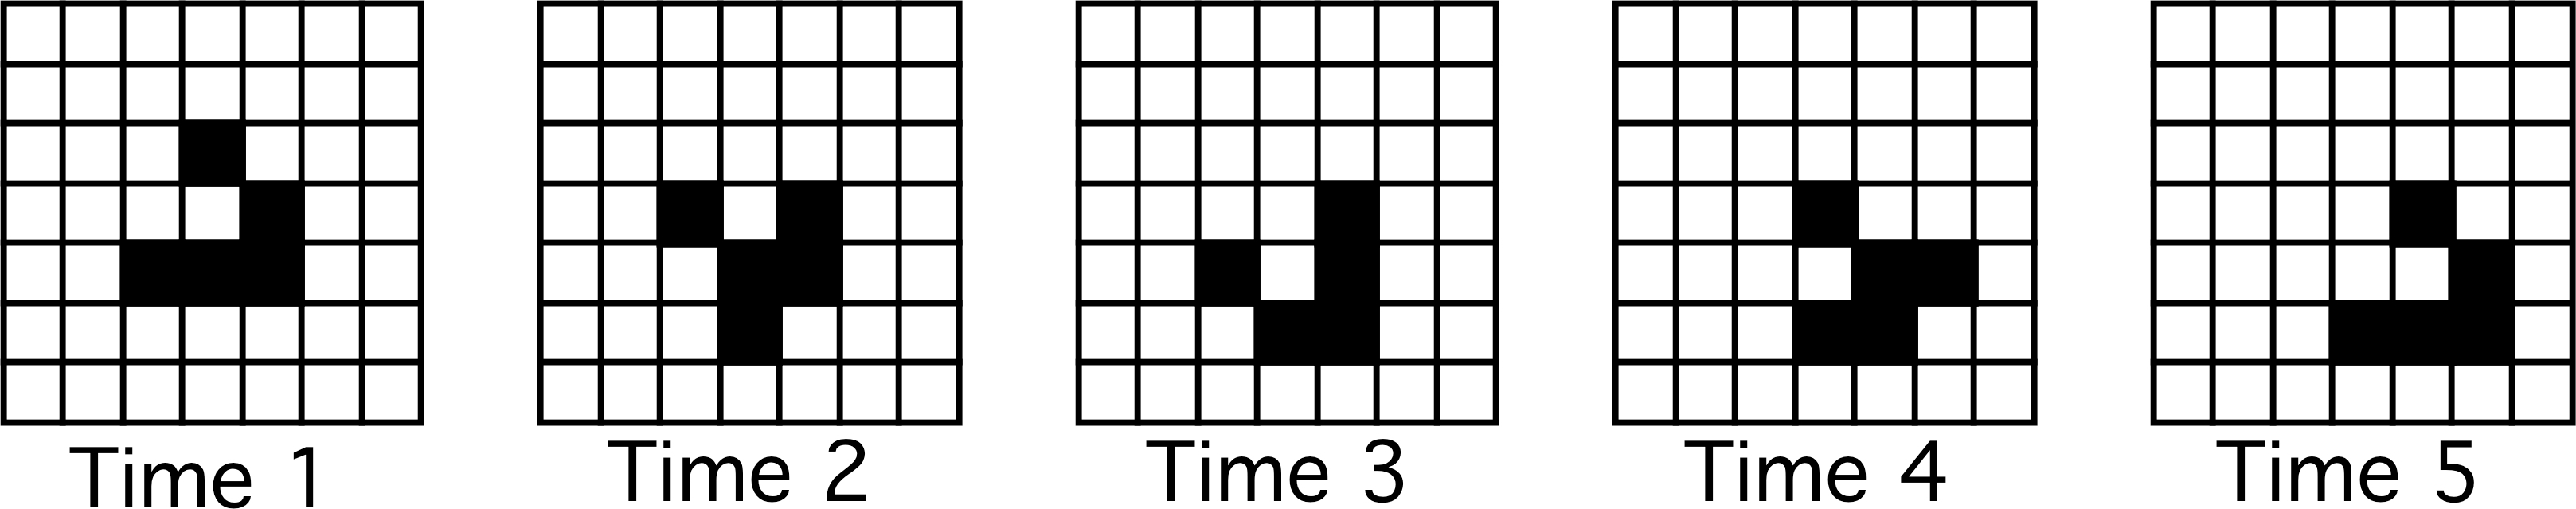
\includegraphics[width=1.0\textwidth]{./images/CA_FDM/glider}}
\end{figure}
This result raises a interesting issue; since the \emph{Halting
Theorem} is undecidable i.e. no algorithm can ever decides whether a Turing Maching will accept a certain input or not,
the evolution of the GOL is \textbf{unpredictable} (as all the universal computational systems) practically meaning that is
not possible to use any algorithmic shortcuts to anticipate the resulting
configuration given an initial input. 
The most efficient way to know the outcome of an execution of GOL, is to let the system run.
\begin{quotation}
\em Life, like all computationally universal systems, defines the most efficient
simulation of its own behavior\cite{Ilachinski2001}
\end{quotation}



\section{Extension of the Cellular automata model - Probabilistic CA}
If some of the assumptions of the ordinary CA characterization are relaxed interesting results are obtained.
As an example, the following are extensions that have proved to be useful in many cases: \textit{asynchronous update}, \textit{non-homogenous cellular space and neighborhood} or  transition function that depends on the coordinates of a cell. An interesting class of CA is obtained when the transition function is based on some stocastic process. 
Probabilistic CA\cite{MAIRESSE201442} have a single key difference w.t.r. to ordinary CA i.e. the transition function $\sigma$ is a stochastic-function that decides the next-state according to some probability distributions.
They are used in a wide class of
problems like in modelling ferromagnetism, statistical mechanics
\cite{Vichniac1984} or the cellular Potts model\footnote{Lattice-based model adopted for the simulation of the collective behavior of cellular structures.}\cite{RevModPhys.54.235}

Probabilistic CA (PCA) evolution can be studied if interpreted as of Markov processes.
A Markov process, is a stochastic process that exhibits
memorylessness, also  called Markov property, which means that the
future state of  a system is conditionally independent from the past.
 Two events $A$ and $B$ are independent if
 $P(A B)=P(A)P(B)$ or in other words, that the probability of the event $A$ to occurs does not depends on the event $B$ i.e. $P(A|B)=P(A)$. 
The property of this kind of  processes allows  future probabilities of an event to be
determined from the probabilities of events at the \textit{current time} only.
In PCA analysis, homogeneous Markov chains are adopted because each cell has a
discrete set of possible value for the status variable.
In terms of such  type of chain a CA is a process that starts in one of these states and moves
successively from one state to another. If the chain is currently in state
$s_i$, than it evolve to state $s_j$ at
the next step with probability $p_{ij}$.The changes of state
of the system are called transitions, and the probabilities associated with
various state changes are named transition probabilities and are usually represented
in the \textit{Markov chain transition matrix} of the form shown below:
\[
M =
\left( {\begin{array}{cccc}
p_{11} & p_{12} & p_{13} &\cdots \\
p_{21} & p_{12} & p_{23} &\cdots \\
p_{31} & p_{32} & p_{33} &\cdots \\
\vdots & \vdots  &\vdots& \ddots\\
\end{array} } \right)
\]
Markov chain transition matrix are useful in analyzing very small PCA but they prove to be impractical for larger sizes as for instance, a
CA on a small celular space of size $10\times10$  has
$2^{10\times10}$ possible states and the resulting chain transition matrix
has size of $2^{10\times10}\times2^{10\times10}$ that is a
huge number! 
